\chapter*{Приложение 1. Результаты обработки изображения <<Лена>>}
\addcontentsline{toc}{chapter}{Приложение 1. Результаты обработки изображения <<Лена>>}
\begin{figure}[h!]
	\centering
	\begin{subfigure}[t]{0.32\textwidth}
		\centering
		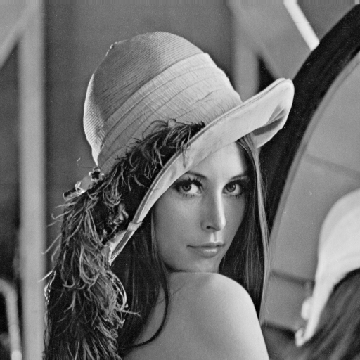
\includegraphics[width=\linewidth]{one-dim-drawn-lena-original}
		\caption{Исходное изображение}
	\end{subfigure}
	\hfill
	\begin{subfigure}[t]{0.32\textwidth}
		\centering
		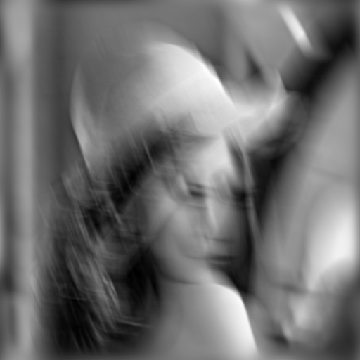
\includegraphics[width=\linewidth]{one-dim-drawn-lena-blurred}
		\caption{смазанное изображение}
	\end{subfigure}
	\hfill
	\begin{subfigure}[t]{0.32\textwidth}
		\centering
		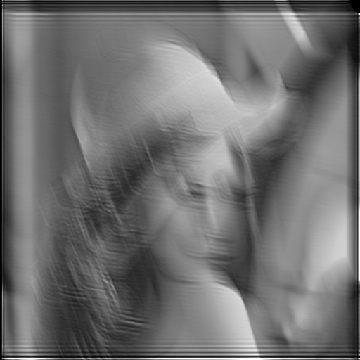
\includegraphics[width=\linewidth]{one-dim-drawn-lena-restored-initial-approx}
		\caption{первое приближение (0; 0), (22.5; 18), (45; 36), PSNR=15.96дБ}
	\end{subfigure}
	\begin{subfigure}[t]{0.32\textwidth}
		\centering
		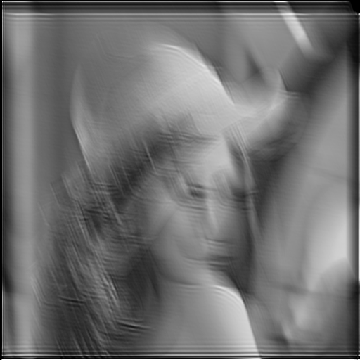
\includegraphics[width=\linewidth]{one-dim-drawn-lena-restored-second-approx}
		\caption{второе приближение (0,0), (4.5; 40.5), (45, 36), PSNR=19.4}
	\end{subfigure}
	\hfill
	\begin{subfigure}[t]{0.32\textwidth}
		\centering
		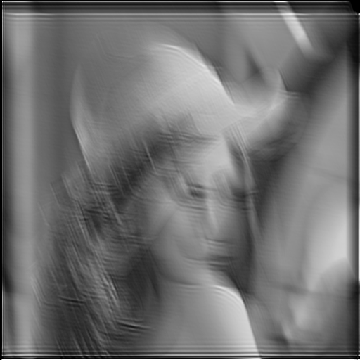
\includegraphics[width=\linewidth]{one-dim-drawn-lena-restored-final}
		\caption{уточнение градиентным спуском (0,0), (4.5; 40.5), (45, 36), PSNR=19.4}
	\end{subfigure}
	\hfill
	\begin{subfigure}[t]{0.32\textwidth}
		\centering
		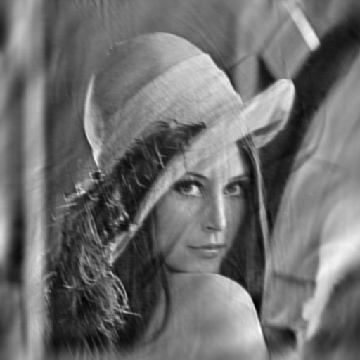
\includegraphics[width=\linewidth]{one-dim-drawn-lena-restored-true-psf}
		\caption{восстановление с <<правильным>> оператором, PSNR=19.4}
	\end{subfigure}
	\label{fig:oneDimDrawnLena}
	\caption{Восстановление изображения искажённого оператором \ref{fig:drawnPsf2}}
\end{figure}

\begin{figure}[h!]
	\centering
	\begin{subfigure}[b]{0.4\textwidth}
		\centering
		
\includegraphics[width=\linewidth]{../input/drawn-psf2}
		\caption{исходный искажающий оператор}
		\label{fig:drawnPsf2}
	\end{subfigure}
	\begin{subfigure}[b]{0.4\textwidth}
		\centering
		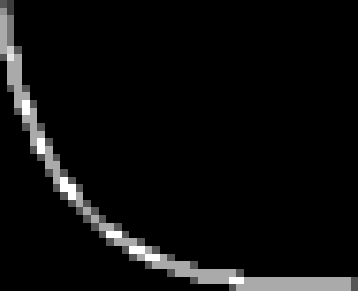
\includegraphics[width=\linewidth]{one-dim-drawn-lena-found-psf}
		\caption{оценка искажающего оператора}
	\end{subfigure}
	\caption{искажающий оператор и его оценка}
\end{figure}
\pagebreak
\chapter*{Приложение 1. Результаты обработки изображения <<Фотограф>>}
\addcontentsline{toc}{chapter}{Приложение 1. Результаты обработки изображения <<Фотограф>>}
\begin{figure}[h!]
	\centering
	\begin{subfigure}[t]{0.32\textwidth}
		\centering
		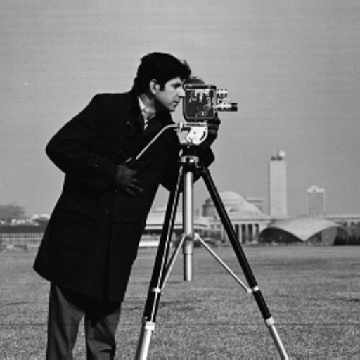
\includegraphics[width=\linewidth]{one-dim-drawn-cameraman-original}
		\caption{Исходное изображение}
	\end{subfigure}
	\hfill
	\begin{subfigure}[t]{0.32\textwidth}
		\centering
		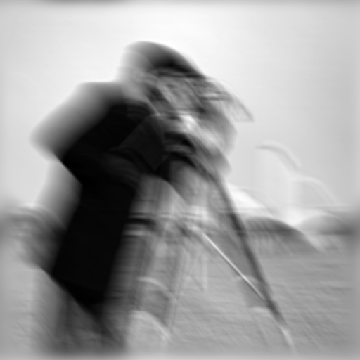
\includegraphics[width=\linewidth]{one-dim-drawn-cameraman-blurred}
		\caption{смазанное изображение}
	\end{subfigure}
	\hfill
	\begin{subfigure}[t]{0.32\textwidth}
		\centering
		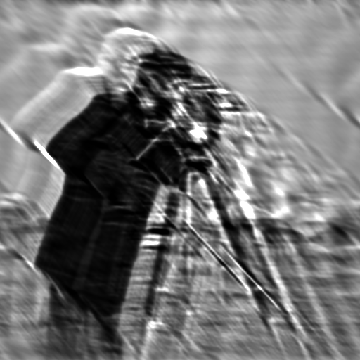
\includegraphics[width=\linewidth]{one-dim-drawn-cameraman-restored-initial-approx}
		\caption{первое приближение (0; 0), (26; 17), (52; 34), PSNR=15.46дБ}
	\end{subfigure}
	\begin{subfigure}[t]{0.32\textwidth}
		\centering
		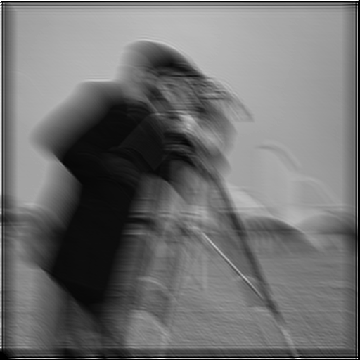
\includegraphics[width=\linewidth]{one-dim-drawn-cameraman-restored-second-approx}
		\caption{второе приближение (0,0), (41.82; -7.21), (52, 34), PSNR=18.22}
	\end{subfigure}
	\hfill
	\begin{subfigure}[t]{0.32\textwidth}
		\centering
		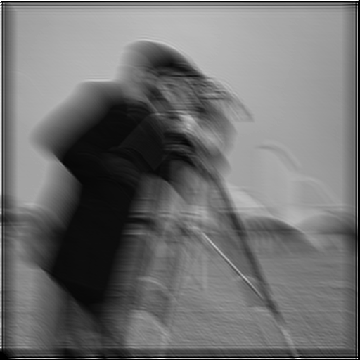
\includegraphics[width=\linewidth]{one-dim-drawn-cameraman-restored-final}
		\caption{уточнение градиентным спуском (0,0), (41.83; -7.61), (51.99, 34.00), PSNR=17.88}
	\end{subfigure}
	\hfill
	\begin{subfigure}[t]{0.32\textwidth}
		\centering
		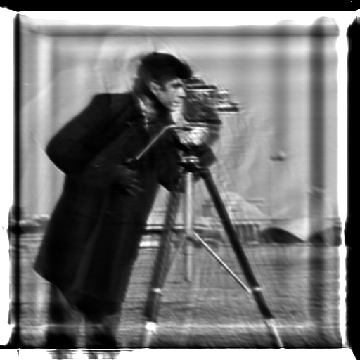
\includegraphics[width=\linewidth]{one-dim-drawn-cameraman-restored-true-psf}
		\caption{восстановление с <<правильным>> оператором, PSNR=21.98}
	\end{subfigure}
	\label{fig:oneDimDrawnCameraman}
	\caption{Восстановление изображения искажённого оператором \ref{fig:drawnPsf3}}
\end{figure}

\begin{figure}[h!]
	\centering
	\begin{subfigure}[b]{0.4\textwidth}
		\centering
		
\includegraphics[width=\linewidth]{../input/drawn-psf3}
		\caption{исходный искажающий оператор}
		\label{fig:drawnPsf3}
	\end{subfigure}
	\begin{subfigure}[b]{0.4\textwidth}
		\centering
		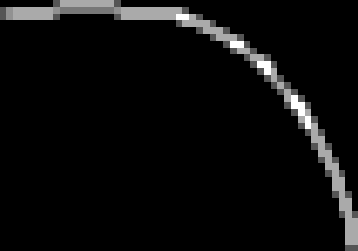
\includegraphics[width=\linewidth]{one-dim-drawn-cameraman-found-psf}
		\caption{оценка искажающего оператора}
	\end{subfigure}
	\caption{искажающий оператор и его оценка}
\end{figure}